\section{Migración}
\subsection{Introducción}

En el apartado de negocio se presenta el modelamiento de los procesos de negocio que son desarrollados dentro de la organización, permitiendo un mayor entendimiento de cada factor que actua en la organización. A medida que se identifican los procesos de negocio en una organización se aprecia que estos, pueden estar operando de la mejor manera o que pueden estar operando con fallas generando pérdidas. La arquitectura de negocio busca ese cambio informando a toda la organización el estado actual y la forma como se llevara a cabo la transformación.


\newpage

\subsection{Punto de Vista de Organización}

El punto de vista de la organización permite identificar los actores, roles y colaboraciones que interactuan en la organización.

%%grafo

\begin{figure}[th!]
	\centering
	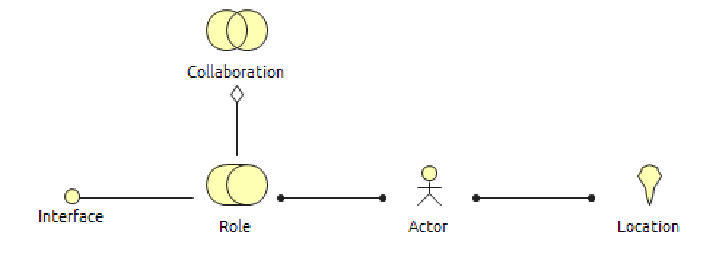
\includegraphics[width=10cm,height=5cm]{arquitectura/negocio/imgs/m_organizacion}
	\caption{Modelo de Organización}{\scriptsize \textbf{Fuente:} Archimate 2.0}
\end{figure}

\subsection{Caso}

En la organización que se presenta dentro de las propiedades horizontales se puede ver roles muy bien definidos.

%%grafo
\begin{figure}[th!]
	\centering
	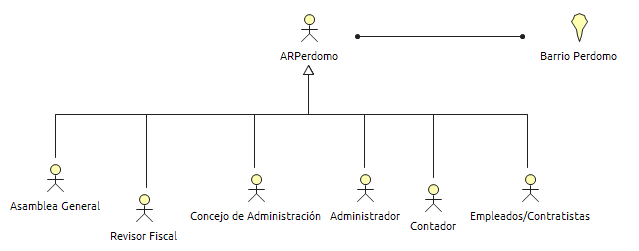
\includegraphics[width=12cm,height=7cm]{arquitectura/negocio/imgs/organizacion}
	\caption{Caso de Organización}{\scriptsize \textbf{Fuente:} Imagen propia}
\end{figure}
\newpage